\begin{exercise}{Arc en ciel}{3}{Sup}
{Réfraction, Optique géométrique}{bermudez}

Un arc-en-ciel se forme lorsqu'un observateur voit par réflection un rideau de gouttes d'eau.

On considère un rayon lumineux qui entre en E sous incidence $i$ dans une goutte d'eau sphérique de rayon $R$ et d'indice optique $n_\text{e}$. Après plusieurs réflections--réfractions, il ressort de la goutte au point S en ayant dévié d'un angle $D$.

La loi de Cauchy établi la relation entre l'indice optique d'un milieu $n$ et la longeur d'onde :
$$n(\lambda) = A + \dfrac{B}{\lambda^2}.$$

\begin{figure}[H]
\centering
\begin{tabular}{rr|ll}
    Milieu & & $A$ & $B$ (nm$^2$)  \\ \hline
    Verre (BK6) & $n_\text{v}$ & $1,5$ & $4\times 10^{3}$ \\
    Eau & $n_\text{e}$ & $1,3$ & $5\times 10^{3}$ \\
    Air & $n_\text{a}$ & $1,0$ & $\sim 0$ \\ \hline
\end{tabular}

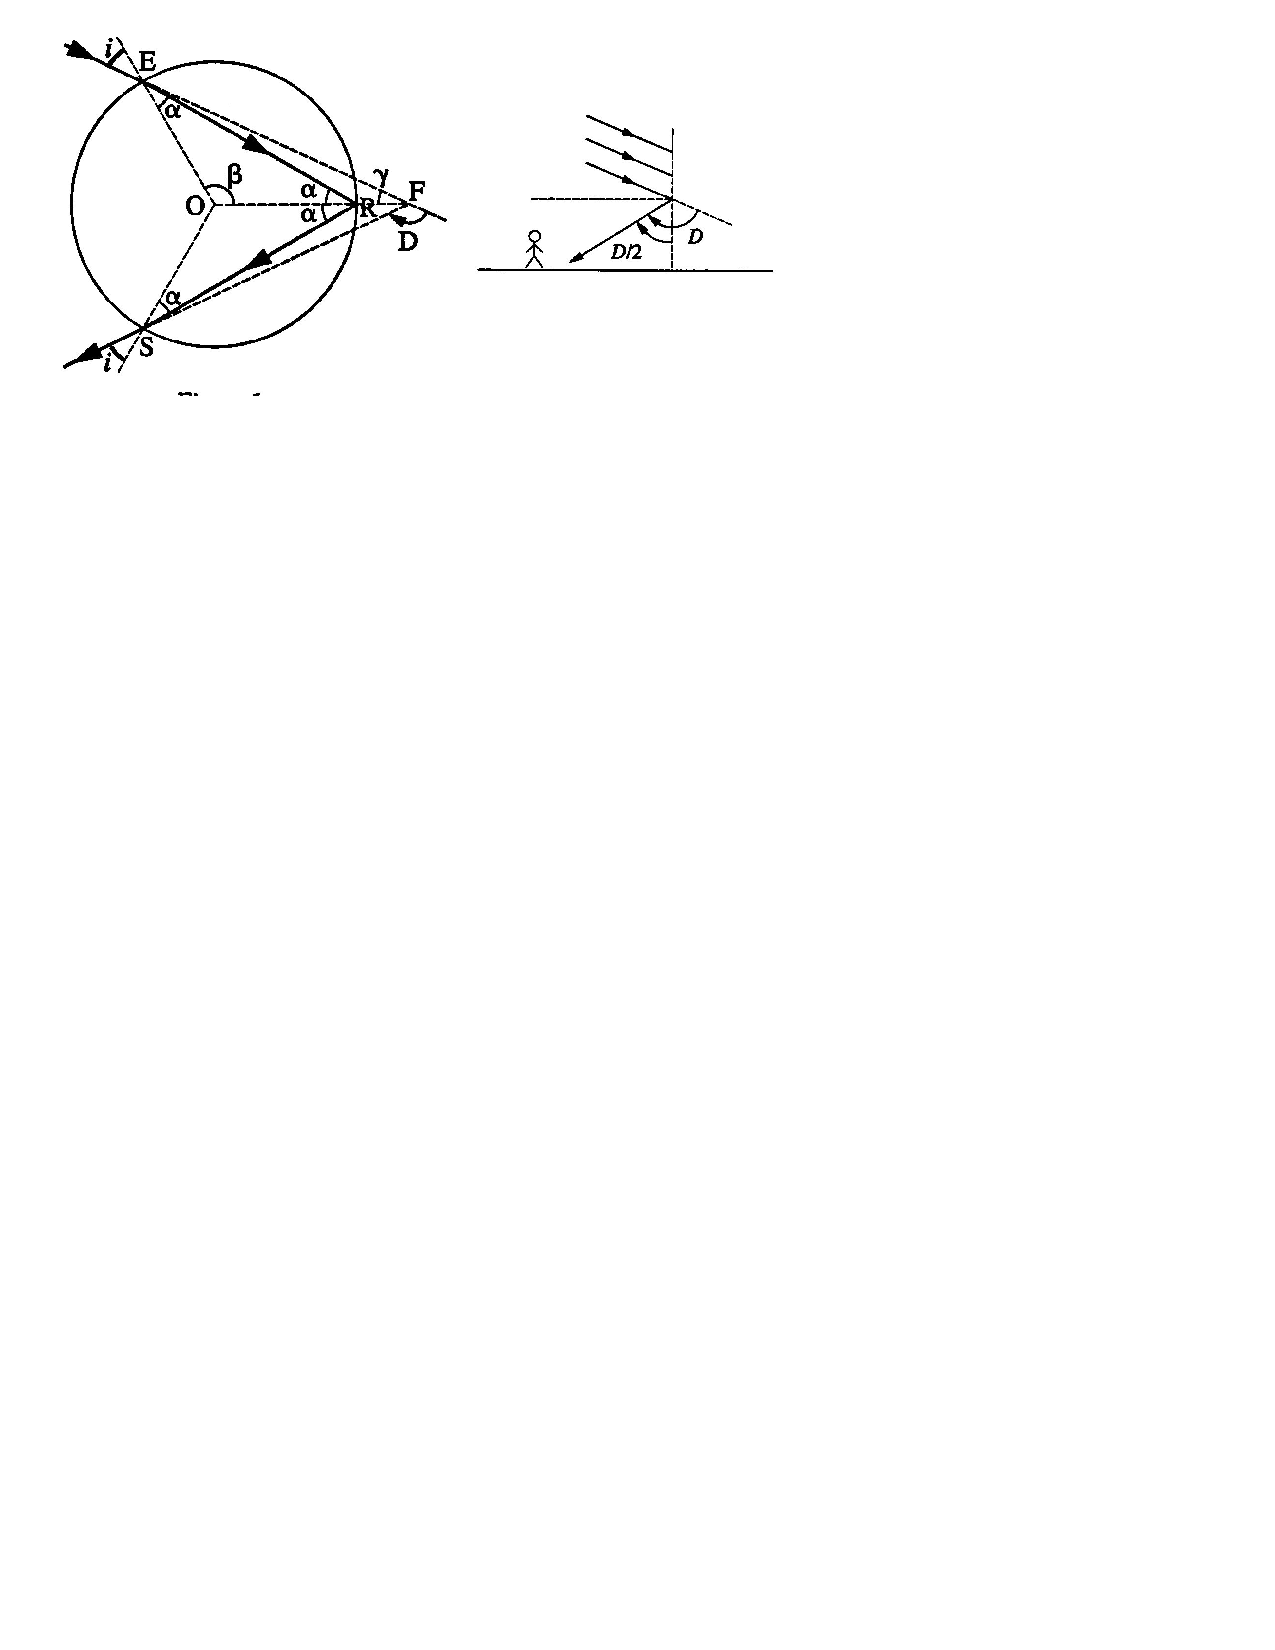
\includegraphics[width=\linewidth]{optique/refraction/arc-en-ciel.pdf}
\end{figure}

\begin{questions}
    \questioncours A l'aide de la loi de Cauchy, expliquer la décomposition de la lumière par un prisme de Newton.
    \question Déterminer l'expression de la déviation $D$ en fonction de l'angle d'incidence $i$ et de l'indice optique de l'eau $n_\text{e}$. \\ On pourra s'aider des angles $\beta$ et $\gamma$ et de leur relations dans les triangles OEF et OER. Et trouver par une autre méthode le lien entre $\alpha$, $i$.
    
    \question Calculer les déviations de part et d'autre du spectre de la lumière visible. On admettra que l'intensité lumineuse maximale est observée pour une incidence de $i = 60^\circ$ (déviation minimale). 
    
    \uplevel{Lorsqu'un rideau de pluie est éclairé par le soleil, un observateur peut voir toutes les couleurs de l'arc-en-ciel. Ce ne sont donc pas les mêmes gouttes qui produisent toutes les couleurs.
    
    Ici l'observateur à $H = 1,00$ km du rideau de pluie.}
    
    \question À quelles altitudes sont situées les gouttes qui produisent chaque extrema de l'arc-en-ciel ?  Que se passe-t-il lorsque l'observateur se rapproche de l'arc-en-ciel ? \\
    On négligera la taille de l'observateur devant l'altitude des gouttes considérées. 
\end{questions}

\end{exercise}
